\section{Ecuaciones en diferencias lineales de orden 1}


\begin{ejercicio} [Depósito de capital]
Un banco ofrece un interés compuesto del $7\%$ anual para depósitos de capital a medio plazo.
    \begin{enumerate}
        \item Si disponemos de un capital inicial de 10000 euros, ¿de qué capital dispondremos al cabo de 4 años?

        En este caso, si $C_n$ denota el capital en el $n-$ésimo año, y el interés es $I=0.07$, tenemos que:
        \begin{equation*}
            C_n = (1+I)^nC_0
        \end{equation*}

        Por tanto, tenemos $C_4=1.07^4\cdot 10^4=13107.96$ euros.
        
        \item Si se pretende disponer de 25000 euros dentro de 4 años, ¿cuál debe ser el capital inicial?

        En este caso, la incógnita es $C_0$. Tenemos:
        \begin{equation*}
            25\cdot 10^3 = 1.07^4 \cdot C_0 \Longrightarrow C_0 = 19072.38 \text{ euros.}
        \end{equation*}
        
        \item Supongamos ahora que no conocemos el interés que proporciona el banco. Si inicialmente disponemos de 10000 euros y pasados 5 años tenemos 12000, ¿cuál es el interés anual aplicado?

        En este caso, tenemos que la incógnita es $I$. Tenemos:
        \begin{equation*}
            12\cdot 10^3 = (1+I)^5\cdot 10\cdot 10^3 \Longrightarrow I = \sqrt[5]{\frac{12}{10}}-1\approx 0.0371
        \end{equation*}

        Por tanto, tenemos que $I\approx 3.71\%$.
    \end{enumerate}
\end{ejercicio}

\begin{ejercicio} [Explosión demográfica]
Una población sigue un modelo de crecimiento malthusiano con tasa de crecimiento neta $\alpha = 0.16$, es decir: si $x_n$ es el número de individuos en el periodo $n$, entonces
$$x_{n+1} = 1.16 x_n.$$
    \begin{enumerate}
        \item Calcula el número de periodos necesarios para que la población se duplique y cuadruplique.

        Tenemos que:
        \begin{equation*}
            x_{n} = 1.16^n x_0
        \end{equation*}

        Calculemos el menor $n\in \bb{N}$ de forma que $1.16^n\geq 2$, que nos indicará el número de periodos necesarios para que la población se duplique.
        Aplicando el logaritmo en base $1.16$, tenemos que:
        \begin{equation*}
            n \geq \log_{1.16} 2 \approx 4.67
        \end{equation*}
        Por tanto, tenemos que el  número de periodos necesarios para que la población se duplique es $n=5$ periodos.
        
        Para el caso de que la población se cuadruplique, necesitamos que $1.16^n \geq 4$. Por tanto,
        \begin{equation*}
            n\geq \log_{1.16} 4 \approx 9.34
        \end{equation*}
        El  número de periodos necesarios para que la población se cuadruplique es $n=10$ periodos.
        
        \item Calcula el tiempo promedio de duplicación.

        En este caso, no se pide un número de periodos, sino el tiempo promedio. En este caso, tenemos que el tiempo medio de duplicación es:
        \begin{equation*}
            \log_{1.16} 2 \approx 4.67
        \end{equation*}
        
        \item Calcula el tiempo promedio de quintuplicación.

        De forma análoga, tenemos que el tiempo medio de quintuplicación es:
        \begin{equation*}
            \log_{1.16} 5 \approx 10.84
        \end{equation*}
    \end{enumerate}
\end{ejercicio}

\begin{ejercicio} [Eliminación de un fármaco en sangre]
Un fármaco se elimina en sangre siguiendo un modelo malthusiano.
Según dicho modelo, su vida media es de 2 semanas.
    \begin{enumerate}
        \item Calcula la concentración inicial de fármaco si a los 5 días encontramos una concentración en sangre de \(3~\nicefrac{mg}{cm^3}\).

        Como la vida media es de 2 semanas, tenemos que:
        \begin{equation*}
            VM = 14 \text{ días} = \frac{1}{1-r} \Longrightarrow r = -\left(\frac{1}{14}-1\right) = \frac{13}{14} \approx 0.9286 
        \end{equation*}

        Sabiendo que $x_5=3$, tenemos que:
        \begin{equation*}
            x_5 = 3 = r^5 x_0 \Longrightarrow x_0 = \frac{3}{r^5} \approx 4.2455~\nicefrac{mg}{cm^3}
        \end{equation*}
        Por tanto, la concentración inicial es de $4.2455~\nicefrac{mg}{cm^3}$.
        
        \item ¿Cada cuánto tiempo se diezma en promedio la concentración de fármaco?

        En este caso, se pide el tiempo promedio para que la concentración sea la décima parte. Tenemos que:
        \begin{equation*}
            x_n = \cancel{x_0}\cdot r^n \geq \frac{\cancel{x_0}}{10} 
        \end{equation*}
        Por tanto, de promedio han de pasar $\log_{r}\frac{1}{10}\approx 31.07$ días para que la concentración se diezme. 
        
        \item Calcula el tiempo necesario para que la concentración de fármaco sea menor que \(0.1~\nicefrac{mg}{cm^3}\).

        Tenemos que:
        \begin{equation*}
            x_n = x_0\cdot r^n < 0.1 
            \Longrightarrow r^n < \frac{0.1}{x_0}
        \end{equation*}
        Por tanto, se pide el primer $n\in \bb{N}$ tal que se cumple eso. Como se tiene que $\log_{r}\frac{0.1}{x_0}\approx 50.89$, han de pasar 51 días.
    \end{enumerate}
\end{ejercicio}

\begin{ejercicio} [Desintegración del carbono$-$14]
Para la datación de los restos arqueológicos se utiliza el isótopo carbono$-$14, porque está presente en los organismos vivos y va desapareciendo de ellos cuando mueren. Esta desintegración se modela mediante la ley malthusiana: 
$$x_{n+1} = r x_n \qquad 0 < r < 1$$
donde cada periodo representa un milenio, \(x_n\) es el número de átomos de carbono$-$14 en el periodo \(n\) y \(r\) es la constante de desintegración radiactiva. Sabemos que la vida media del carbono$-$14 se estima en $5730$ años.
    \begin{enumerate}
        \item En un monte se han encontrado restos arqueológicos de una determinada especie. Sabiendo que la cantidad de carbono$-$14 de los restos, en el momento del hallazgo, corresponde al $15.27\%$ de la cantidad que tiene un cuerpo vivo, determina la antigüedad de los restos hallados.

        Como la vida media del carbono$-$14 se estima en $5730$ años ($5.73$ milenos), tenemos que:
        \begin{equation*}
            VM = 5.73 \text{ milenios } = \frac{1}{1-r} \Longrightarrow
            r = -\left(\frac{1}{5.73}-1\right) \approx 0.825 
        \end{equation*}
        donde hemos usado milenios ya que es la unidad del periodo.

        Sabemos que $x_n = r^n x_0$, y se pide el valor de $n$ tal que $x_n = 0.1527x_0$. Por tanto,
        \begin{equation*}
            0.1527 \cancel{x_0} = r^n \cancel{x_0}
        \end{equation*}

        Como $\log_{r}0.1527 \approx 9.7986$ milenios, tenemos que la antigüedad es de 9798 años.
        
        \item ¿Qué tanto por ciento de la cantidad de carbono$-$14 que tiene un cuerpo vivo debe tener un resto arqueológico de aproximadamente $1000$ años de antigüedad?

        Como $1000$ años equivale a un milenio, nos piden calcular $\frac{x_1}{x_0}$. Tenemos que:
        \begin{equation*}
            x_1 = rx_0 \Longrightarrow \frac{x_1}{x_0}=r\approx 0.825 \approx 82.5\%
        \end{equation*}
    \end{enumerate}
\end{ejercicio}

\begin{ejercicio} En un hospital está llevándose a cabo un estudio sobre una enfermedad rara. Para ello se supone que la enfermedad desaparece siguiendo un modelo malthusiano al aplicarle un determinado fármaco. Los datos de que se disponen son los siguientes:
    \begin{itemize}
        \item Fueron puestos en observación 20 pacientes afectados por dicha enfermedad.
        \item Transcurridos 7 días, la mitad de personas ingresadas con motivo de la enfermedad fueron dadas de alta.
    \end{itemize}
    
    ¿Qué puede decirse del modelo propuesto si tras 25 días (desde que se inició la observación de las 20 personas) hay 3 personas que aún no han superado la enfermedad?\\

    Sea $x_n$ la variable que representa el número de pacientes que no han superado la enfermedad en el día $n$. Tenemos que:
    \begin{equation*}
        x_0 = 20 \qquad x_7 = 10 \qquad x_{25} = 3
    \end{equation*}

    Como sabemos sigue un modelo malthusiano, tenemos que $x_n = r^nx_0$. Veamos cuánto vale $r$.
    \begin{align*}
        x_7 &= 10 = r^7\cdot 20
        \Longrightarrow
        r^7 = \frac{1}{2} \Longrightarrow
        r = \frac{1}{\sqrt[7]{2}}\approx 0.9057
    \end{align*}

    Veamos si el modelo de Malthus predice correctamente el valor de $x_{25}$:
    \begin{equation*}
        x_{25} = r^{25}x_0 \approx 1.6823
    \end{equation*}

    Como en la realidad se da que $x_{25}=3$, tenemos que en realidad el Modelo de Malthus no es idóneo para este fármaco.
\end{ejercicio}


\begin{ejercicio}
    Una apicultora de la Alpujarra está estudiando el comportamiento de sus abejas. Ha observado que se distribuyen entre el romero y el tomillo en primavera. Empíricamente ha observado que cada día cambian de unas flores a otras de la siguiente forma:
    \begin{itemize}
        \item El $75\%$ de las abejas que están en las flores de romero en un determinado día permanecen en ellas al día siguiente, mientras que el resto cambia a las flores de tomillo.

        \item El $50\%$ de las abejas que están en las flores de tomillo en un determinado día permanecen en ellas al día siguiente, mientras que el resto cambia a las flores de romero.
    \end{itemize}

    Al comienzo de su estudio había 3400 abejas en las flores de romero y 2600 en las de tomillo. La apicultora pretende estudiar cómo evoluciona la población de abejas en relación con las dos clases de flores, para lo cual llama $x_n$ al número de abejas que hay en el romero en el $n-$ésimo día e $y_n$ al número de abejas que hay en el tomillo en el $n-$ésimo día.

    \begin{enumerate}
        \item Escribe las leyes de recurrencia que modelan la cantidad de abejas en cada tipo de flor según las observaciones de la apicultora.

        Tenemos la siguiente situación:
        \begin{figure}[H]
            \centering
            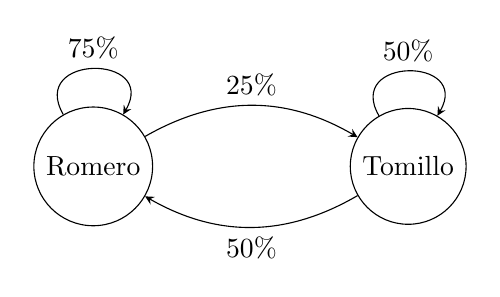
\begin{tikzpicture}
                \node[draw, circle] (A) at (-2,0) {Romero};
                \node[draw, circle] (B) at (2,0) {Tomillo};
                
                \draw[-stealth, bend left] (A) to node[midway, above] {$25\%$} (B);
                \draw[-stealth, bend left] (B) to node[midway, below] {$50\%$} (A);
                
                \draw[-stealth] (A) to [out=120,in=60,looseness=3] node[midway, above] {$75\%$} (A);
                \draw[-stealth] (B) to [out=120,in=60,looseness=3] node[midway, above] {$50\%$} (B);
            \end{tikzpicture}
        \end{figure}

        \begin{itemize}
            \item Sea $x_n$ el número de abejas en romero en el $n$-ésimo día.
            \item Sea $y_n$ el número de abejas en tomillo en el $n$-ésimo día.
        \end{itemize}

        La ley de recurrencia que modela la cantidad de abejas en el romero es:
        $$\left\{\begin{array}{ll}
            x_{n+1} = x_n - 0.25x_n + 0.5y_n \\
            x_0 = 3400
        \end{array}\right.$$

        La ley de recurrencia que modela la cantidad de abejas en el tomillo es:
        $$\left\{\begin{array}{ll}
            y_{n+1} = y_n - 0.5y_n + 0.25x_n \\
            y_0 = 2600
        \end{array}\right.$$
        
        \item Demuestra que $x_n + y_n = 6000$.

        Demostramos por inducción sobre $n$:
        \begin{itemize}
            \item \ul{Caso base $n=1$}:

            Tenemos que:
            $$x_1 = x_0 - 0.25x_0 + 0.5y_0$$
            $$y_1 = y_0 - 0.5y_0 + 0.25x_0$$

            Por tanto, se tiene:
            \begin{align*}
            x_1+y_1 &= x_0 - \cancel{0.25x_0} + \cancel{0.5y_0}+y_0-\cancel{0.5y_0}+\cancel{0.25x_0} \\
                &= x_0 + y_0 = 3400 + 2600 = 6000
            \end{align*}

            \item \ul{Supuesto cierto para $n$, lo demostramos para $n+1$}:
            \begin{align*}
                x_{n+1} + y_{n+1} = x_n - \cancel{0.25x_n} + \cancel{0.5y_n} + y_n - \cancel{0.5y_n} + \cancel{0.25x_n} = x_n + y_n \AstIg 6000
            \end{align*}
            donde en $(\ast)$ hemos empleado la hipótesis de inducción.
        \end{itemize}
        
        \item Escribe una ecuación en diferencias para $x_n$ y resuélvela.

        Como $x_n+y_n=6000$, tenemos que $y_n = 6000 - x_n$. Por tanto, de la Ley de Recurrencia calculada antes, deducimos que:
        \begin{align*}
            x_{n+1} &= 0.75x_n + 0.5y_n
            = 0.75x_n + 0.5\left(6000 - x_n\right)
            =\\&= 0.75x_n + 3000 - 0.5 x_n =\\&= 0.25x_n + 3000
        \end{align*}

        Para resolverla, por lo visto en teoría sabemos que:
        \begin{align*}
            x_n &= 0.25^n x_0 + 3000\cdot \frac{1-0.25^n}{1-0.25} = 0.25^n x_0 + 4000\cdot\left(1-0.25^n\right)
            =\\&= 0.25^n x_0 + 4000 - 4000\cdot 0.25^n = 0.25^n \left(x_0-4000\right) + 4000
        \end{align*}
        
        \item Determina el comportamiento asintótico de la población de abejas en ambas flores.

        $$\lim_{n\to \infty}x_n = \lim_{n\to \infty}  0.25^n \left(x_0-4000\right) + 4000 = 4000$$
        Por tanto, se quedarán $4000$ en el romero y $2000$ en el tomillo.    
    \end{enumerate}
\end{ejercicio}





\begin{ejercicio}
    Dos países, A y B, compiten por el abastecimiento del crudo mundial. Se sabe que el país A cuida más a su clientes y, por tanto, el $90\%$ de quienes un año contratan el abastecimiento con dicho país vuelven a hacerlo el año siguiente. Sin embargo, solo el $70\%$ de los clientes de B vuelven a concertar de nuevo su abastecimiento con este país. Se supone que todos los países tienen que contratar su abastecimiento con A o con B. Este año la situación política del país A impide que pueda abastecer a ningún otro país. ¿Cómo evolucionarán a partir de ahí las cuotas de mercado, es decir, el número de países que contratan el abastecimiento con A y con B medido en tanto por uno?\\

    Tenemos la siguiente situación:
    \begin{figure}[H]
        \centering
        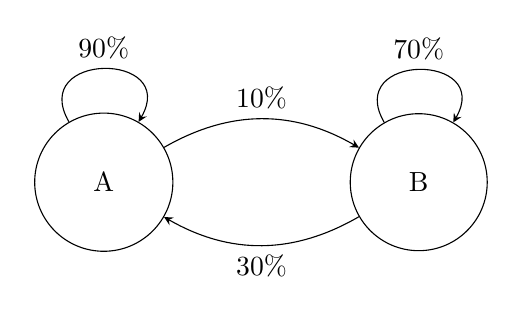
\begin{tikzpicture}
            \node[draw, circle] (A) at (-2,0) {{\color{white}.}\hspace{0.5cm}A\hspace{0.5cm}{\color{white}.}};
            \node[draw, circle] (B) at (2,0) {{\color{white}.}\hspace{0.5cm}B\hspace{0.5cm}{\color{white}.}};
            
            \draw[-stealth, bend left] (A) to node[midway, above] {$10\%$} (B);
            \draw[-stealth, bend left] (B) to node[midway, below] {$30\%$} (A);
            
            \draw[-stealth] (A) to [out=120,in=60,looseness=3] node[midway, above] {$90\%$} (A);
            \draw[-stealth] (B) to [out=120,in=60,looseness=3] node[midway, above] {$70\%$} (B);
        \end{tikzpicture}
    \end{figure}

    \begin{itemize}
        \item Sea $a_n$ los clientes del país $A$ en el año $n$.
        \item Sea $b_n$ los clientes del país $B$ en el año $n$.
    \end{itemize}

    Las leyes de recurrencia que modelan ambos datos son:
    \begin{align*}
        a_{n+1} &= 0.9a_n + 0.3b_n\\
        b_{n+1} &= 0.7b_n +0.1a_n
    \end{align*}

    Además, sabemos que $a_n+b_n=1$ para todo $n\in \bb{N}$, ya que se reparten la totalidad del mercado en tanto por cierto. Por hipótesis, tenemos también que $a_0=0$, $b_0=1$. Como $b_n=1-a_n$, tenemos que:
    \begin{align*}
        a_{n+1} = 0.9a_n + 0.3(1-a_n) = 0.6a_n + 0.3
    \end{align*}

    Por lo visto en teoría, tenemos que:
    \begin{equation*}
        a_n = \left(a_0-\frac{0.3}{1-0.6}\right)\cdot 0.6^n + \frac{0.3}{1-0.6}
        = -\frac{0.3}{0.4}\cdot 0.6^n + \frac{0.3}{0.4}
        = 0.75\left(1-0.6^n\right)
    \end{equation*}

    Por tanto, se tiene que:
    \begin{equation*}
        b_n = 1-a_n = 0.25 + 0.75\cdot 0.6^n
    \end{equation*}

    A largo plazo, cuando $n\to \infty$, se tiene que:
    \begin{equation*}
        \lim_{n\to \infty} a_n = 0.75
        \qquad 
        \lim_{n\to \infty} b_n = 0.25
    \end{equation*}
\end{ejercicio}


\begin{ejercicio}
    Las compañías Paga$+$ y Paga$-$ se han repartido el mercado de la telefonía. A pesar de la agresiva campaña desarrollada por Paga$+$, Paga$-$ viene consiguiendo una mayor fidelización. Se ha observado que cada año el $25\%$ de los clientes de Paga$-$ se pasan a Paga$+$, mientras que el $50\%$ de los de Paga$+$ cambian a Paga$-$. ¿Qué se puede decir sobre el mercado de la telefonía a largo plazo?\\

    Tenemos la siguiente situación:
    \begin{figure}[H]
        \centering
        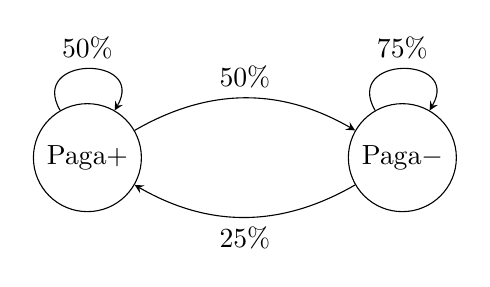
\begin{tikzpicture}
            \node[draw, circle] (A) at (-2,0) {Paga$+$};
            \node[draw, circle] (B) at (2,0) {Paga$-$};
            
            \draw[-stealth, bend left] (A) to node[midway, above] {$50\%$} (B);
            \draw[-stealth, bend left] (B) to node[midway, below] {$25\%$} (A);
            
            \draw[-stealth] (A) to [out=120,in=60,looseness=3] node[midway, above] {$50\%$} (A);
            \draw[-stealth] (B) to [out=120,in=60,looseness=3] node[midway, above] {$75\%$} (B);
        \end{tikzpicture}
    \end{figure}

    \begin{itemize}
        \item Sea $x_n$ el número de clientes de Paga$+$ en el año $n$-ésimo.
        \item Sea $y_n$ el número de clientes de Paga$-$ en el año $n$-ésimo.
    \end{itemize}

    Las leyes de recurrencia que modelan ambos datos son:
    \begin{gather*}
        x_{n+1} = 0.5x_n + 0.25y_n \\
        y_{n+1} = 0.5x_n + 0.75y_n
    \end{gather*}

    Como se han repartido la totalidad del mercado, tenemos que $x_n + y_n = 1$ para todo $n\in \bb{N}$ (ver observación debajo). Por tanto:
    \begin{gather*}
        x_{n+1} = 0.5x_n + 0.25y_n = 0.5x_n +0.25(1-x_n) = 0.25x_n + 0.25
    \end{gather*}

    Por tanto, la solución de este modelo es:
    \begin{equation*}
        x_n = 0.25^nx_0 + 0.25\cdot \frac{1-0.25^n}{0.75} = 0.25^nx_0 + \frac{1-0.25^n}{3}
    \end{equation*}

    Tomamos límite para ver el comportamiento del mercado a largo plazo:
    $$\lim_{n \to \infty} x_n = \lim_{n \to \infty} 0.25^nx_0 + \frac{1-0.25^n}{3} = \dfrac{1}{3}$$
    Por tanto, se tiene que:
    $$\lim_{n \to \infty} y_n = \dfrac{2}{3}$$
    En conclusión, el número de empleados de Paga$+$ se establecerá en el $33\%$ del total del mercado, mientras que Paga$-$ en el $66\%$ del total del mercado.
    
\begin{observacion}
    Notemos que la elección de $x_n + y_n = 1$ es insignificante: ante cualquier constante obtendríamos el mismo resultado. Esto se debe a que se trata de un sistema ``cerrado'', ningún cliente sale de las dos compañías al mismo tiempo y tampoco tenemos clientes nuevos que se apunten a alguna y no estuvieran apuntados antes.   

    Esto nos permite fijar un valor cualesquiera para $x_n + y_n$ constante.
\end{observacion}
        
\end{ejercicio}


\begin{ejercicio}
    Una jugadora de ajedrez es contratada por la compañía Galactic Chess. Su trabajo consiste en jugar 40 partidas simultáneas cada semana. La jugadora dispone de dos estrategias, A y B. Gana en el $80\%$ de los casos con la estrategia A y en el $60\%$ de los casos con la B. Para diversificar su juego decide que cada semana empleará la estrategia B tantas veces como derrotas o tablas haya cosechado la semana anterior. Después de algunas semanas de practicar este sistema observa que siempre acaba jugando el mismo número de partidas con la estrategia B. ¿Cómo se explica este hecho?

    \begin{itemize}
        \item Sea $a_n$ el número de partidas que se juegan la semana $n$ con la estrategia $A$.
        \item Sea $b_n$ el número de partidas que se juegan la semana $n$ con la estrategia $B$.
        \item Sea $g_n$ el número de partidas ganadas en la semana $n$.
    \end{itemize}

    Veremos dos formas de plantear el ejercicio:
    \begin{description}
        \item[Opción 1.]~

        Sabemos que $a_n+b_n=40$ para todo $n\in \bb{N}$. Además, tenemos que:
        \begin{equation*}
            g_n = 0.8a_n + 0.6b_n = 0.8(40-b_n) + 0.6b_n = 32-0.2b_n
        \end{equation*}
    
        Como cada semana juega con la estrategia $B$ tantas partidas como derrotas o tablas (no victorias) haya cosechado la semana anterior, tenemos que $b_n = 40-g_{n-1}$. Por tanto,
        \begin{equation*}
            g_n = 32-0.2\cdot (40-g_{n-1})
            = 24+0.2g_{n-1}
        \end{equation*}
    
        La solución por tanto de dicha recurrencia es:
        \begin{equation*}
            g_n = \left(x_0-\frac{24}{1-0.2}\right)0.2^n + \frac{24}{1-0.2}
            = \left(x_0-30\right)0.2^n + 30
        \end{equation*}
    
        Para $n\to \infty$, tenemos que $\{g_n\}\to 30$, por lo que el número de partidas perdidas en tablas se estabilizará en 10, que será el número de partidas que jugará con la estrategia B.

        \item[Opción 2.]~
    
        Tenemos entonces que:
        \begin{align*}
            &a_n + b_n = 40 \Longrightarrow a_n = 40 - b_n\\
            &b_{n+1} = 0.2a_n + 0.4b_n
        \end{align*}
        
        Combinando las dos:
        \begin{align*}
            b_{n+1} &= 0.2a_n + 0.4b_n = 0.2(40-b_n) + 0.4b_n \\
            &= 0.2b_n + 8
        \end{align*}
        
        La solución de dicha recurrencia nos es conocida:
        \begin{equation*}
            b_n = 0.2^n b_0 + 8 \frac{1-0.2^n}{1-0.2} = 0.2^n b_0 + 10(1-0.2^n)
        \end{equation*}
        Para $n\to \infty$, tenemos que $\{b_n\}\to 10$, el número en el que se estabilizará el número de partidas a partir de una en adelante.
    \end{description}

    

    
\end{ejercicio}


\begin{ejercicio}
    Una compañía maderera tala el $10\%$ de un bosque anualmente. Para compensar el perjuicio causado, cada año se planta un número fijo de árboles K. Si no se tienen en cuenta otros condicionantes:
    \begin{enumerate}
        \item Escribe la ley de recurrencia que modela el tamaño del bosque.

        Tenemos que:
        \begin{equation*}
            x_{n+1} = x_n + K - 0.1x_n = 0.9x_n + K
        \end{equation*}
        
        \item Si el tamaño inicial del bosque es de 10000 árboles, calcula la solución de la ecuación del modelo.

        \begin{description}
            \item[Opción 1.] Demostramos mediante inducción que:
            \begin{equation*}
                x_n = 0.9^n \cdot x_0 + \sum_{i=0}^{n-1}(0.9^iK)
            \end{equation*}
            \begin{itemize}
                \item \ul{Para $n=1$}:
                \begin{equation*}
                    x_1 = 0.9\cdot x_0 + K
                \end{equation*}
    
                \item \ul{Supuesto cierto para $n$, demostramos para $n+1$}:
                \begin{align*}
                    x_{n+1} &= 0.9x_n + K =
                    0.9\left[0.9^nx_0 + \sum_{i=0}^{n-1}0.9^iK\right] + K
                    =\\&= 0.9^{n+1}x_0 + \sum_{i=1}^{n}0.9^iK + K
                    = 0.9^{n+1}x_0 + \sum_{i=0}^{n}0.9^iK
                \end{align*}
            \end{itemize}
    
            Por tanto, resolviendo la suma, tenemos que:
            \begin{align*}
                x_n &= 0.9^n\cdot x_0 + K\sum_{i=0}^{n-1}0.9^i
                = 0.9^n\cdot x_0 + K\cdot \frac{1-0.9^n}{1-0.9}
                =\\&= 0.9^nx_0 + 10K(1-0.9^n)
            \end{align*}

            \item[Opción 2.] Notando $a=0.9$ y $b=K$, por lo visto en teoría sabemos que:
            \begin{equation*}
                x_n = \left(x_0-\frac{b}{1-a}\right)a^n + \frac{b}{1-a}
                = (x_0-10K)0.9^n + 10K
            \end{equation*}
        \end{description}

        
        \item Si plantar un árbol tiene un coste de 1 euro, calcula el precio mínimo al que deben venderse los árboles talados para que la explotación sea rentable a largo plazo.\\

        Veamos en primer lugar cuántos árboles hay a largo plazo. Tenemos que:
        \begin{equation*}
            \lim_{n\to \infty} x_n = \lim_{n\to \infty}
            (x_0-10K)0.9^n + 10K = 10K
        \end{equation*}

        Sea $v$ el precio de venta, y notemos por $v_n$ las ganancias en el periodo $n$. Tenemos que:
        \begin{equation*}
            v_n = 0.1vx_n -1\cdot K
        \end{equation*}

        Como se busca que sea rentable a largo plazo, necesitamos que:
        \begin{equation*}
            \lim_{n\to \infty} v_n
            = \lim_{n\to \infty} 0.1vx_n -1\cdot K
            = 0.1v\cdot 10K - K = vK -K=K(v-1) > 0 \Longleftrightarrow v>1
        \end{equation*}

        Por tanto, para que no haya pérdidas a largo plazo el precio mínimo es $v=1$.
    \end{enumerate}
\end{ejercicio}


\begin{ejercicio} \label{ej:1.11}
    Los precios de cierto producto siguen una dinámica basada en los postulados del modelo de la telaraña con funciones de oferta y demanda dadas por
    \begin{equation*}
        O(p)=1+p,\qquad D(p)=2-2p.
    \end{equation*}
    Suponemos que el equilibrio de mercado se alcanza cuando la oferta iguala a la demanda y que la oferta en el periodo $(n + 1)-$ésimo depende del precio de equilibrio $n-$ésimo.
    \begin{enumerate}
        \item Deduce la ecuación en diferencias que describe la dinámica planteada y calcula el precio de mercado $p^\ast$ (punto de equilibrio económicamente factible).\\

        Sea $p_n$ la sucesión que determina el precio en el mercado en el periodo $n$. Tenemos que la ecuación en diferencias a calcular es $O(p_{n})=D(p_{n+1})$, es decir:
        \begin{equation*}
            1+p_n = 2-2p_{n+1} \Longrightarrow p_{n+1} = -\frac{1}{2}p_n +\frac{1}{2}
        \end{equation*}

        El precio de equilibrio $p^\ast$ es la solución constante de dicha solución, es decir:
        \begin{equation*}
            p^\ast = -\frac{1}{2}p^\ast +\frac{1}{2} \Longrightarrow \frac{3}{2}p^\ast = \frac{1}{2}
            \Longrightarrow p^\ast = \frac{1}{3}
        \end{equation*}

        Por tanto, tenemos que el precio de equilibrio es $p^\ast = \frac{1}{3}$ euros.
        
        \item ¿Cuál es la tendencia del precio del producto a largo plazo?\\

        La solución de la ecuación en diferencias sabemos que es:
        \begin{equation*}
            p_{n} = (p_0-p^\ast)\cdot \left(\frac{-1}{2}\right)^n + p^\ast
        \end{equation*}

        Como $\left|\nicefrac{-1}{2}\right|<1$, tenemos que $\{p_n\}\to p^\ast$, es decir, a largo plazo el precio se estabiliza en el precio de equilibrio. Sabemos además que lo hace oscilando.
        
        \item Analiza gráficamente la evolución de los precios.

        \begin{figure}[H]
            \centering
            \begin{tikzpicture}
                \begin{axis}[
                    axis lines = center,
                    ylabel = $p$,
                    legend pos=outer north east
                ]
                
                % Curva de oferta
                \addplot[domain=-0.5:2, samples=100, color=red]{1+x}; 
                \addlegendentry{$O(p)$}
                
                % Curva de demanda
                \addplot[domain=-0.5:2, samples=100, color=blue]{2-2*x}; 
                \addlegendentry{$D(p)$}
                
                % Trayectoria de la telaraña
                \draw[dashed, -stealth] (0,1) -- (0.5, 1);
                \draw[dashed, -stealth] (0.5, 1) -- (0.5, 1.5);
                \draw[dashed, -stealth] (0.5, 1.5) -- (0.25, 1.5);
                \draw[dashed, -stealth] (0.25, 1.5) -- (0.25, 1.25);
                \draw[dashed, -stealth] (0.25, 1.25) -- (0.375, 1.25);
                \draw[dashed, -stealth] (0.375, 1.25) -- (0.375, 1.375);
                \addlegendentry{Telaraña}
    
                \node at (axis cs:0.33333,1.33333) [pin=45:{$p^\ast$},inner sep=0pt] {};

                \end{axis}
            \end{tikzpicture}
            \caption{Representación del modelo de la Telaraña para el ejercicio \ref{ej:1.11}.}
        \end{figure}
    \end{enumerate}
\end{ejercicio}

\begin{ejercicio} \label{ej:1.12}
    Resuelve el Ejercicio \ref{ej:1.11} para el caso en que las funciones de oferta y demanda vienen dadas por
    \begin{equation*}
        O(p)=1+p,\qquad D(p)=2-0.5p.
    \end{equation*}

    Suponemos que el equilibrio de mercado se alcanza cuando la oferta iguala a la demanda y que la oferta en el periodo $(n + 1)-$ésimo depende del precio de equilibrio $n-$ésimo.
    \begin{enumerate}
        \item Deduce la ecuación en diferencias que describe la dinámica planteada y calcula el precio de mercado $p^\ast$ (punto de equilibrio económicamente factible).\\

        Sea $p_n$ la sucesión que determina el precio en el mercado en el periodo $n$. Tenemos que la ecuación en diferencias a calcular es $O(p_{n})=D(p_{n+1})$, es decir:
        \begin{equation*}
            1+p_n = 2-0.5p_{n+1} \Longrightarrow p_{n+1} = -2p_n +2
        \end{equation*}

        El precio de equilibrio $p^\ast$ es la solución constante de dicha solución, es decir:
        \begin{equation*}
            p^\ast = -2p^\ast +2 \Longrightarrow p^\ast = \frac{2}{3}
        \end{equation*}

        Por tanto, tenemos que el precio de equilibrio es $p^\ast = \frac{2}{3}$ euros.
        
        \item ¿Cuál es la tendencia del precio del producto a largo plazo?\\

        La solución de la ecuación en diferencias sabemos que es:
        \begin{equation*}
            p_{n} = (p_0-p^\ast)\cdot \left(-2\right)^n + p^\ast
        \end{equation*}

        Como $\left|-2\right|>1$, tenemos que $\{|p_n|\}\to +\infty$, es decir, a largo plazo el precio se dispara. No tiene sentido considerarlo.
        
        \item Analiza gráficamente la evolución de los precios.

        \begin{figure}[H]
            \centering
            \begin{tikzpicture}
                \begin{axis}[
                    axis lines = center,
                    ylabel = $p$,
                    legend pos=outer north east
                ]
                
                % Curva de oferta
                \addplot[domain=-5:5, samples=100, color=red]{1+x}; 
                \addlegendentry{$O(p)$}
                
                % Curva de demanda
                \addplot[domain=-5:5, samples=100, color=blue]{2-0.5*x}; 
                \addlegendentry{$D(p)$}
                
                % Trayectoria de la telaraña
                \draw[dashed, -stealth] (0,1) -- (2, 1);
                \draw[dashed, -stealth] (2, 1) -- (2,3);
                \draw[dashed, -stealth] (2,3) -- (-2,3);
                \draw[dashed, -stealth] (-2,3) -- (-2,-1);
                \draw[dashed, -stealth] (-2,-1) -- (6,-1);
                \draw[dashed, -stealth] (6,-1) -- (6,7);
                \addlegendentry{Telaraña}
    
                %\node at (axis cs:0.33333,1.33333) [pin=45:{$p^\ast$},inner sep=0pt] {};

                \end{axis}
            \end{tikzpicture}
            \caption{Representación del modelo de la Telaraña para el ejercicio \ref{ej:1.12}.}
        \end{figure}
        Como podemos ver, claramente el precio se dispara, oscilando entre valores positivos y negativos.
    \end{enumerate}
\end{ejercicio}

\begin{ejercicio} \label{ej:1.13}
    Resuelve el Ejercicio \ref{ej:1.11} para el caso en que las funciones de oferta y demanda vienen dadas por
    \begin{equation*}
        O(p)=1+p,\qquad D(p)=2-p.
    \end{equation*}

    Suponemos que el equilibrio de mercado se alcanza cuando la oferta iguala a la demanda y que la oferta en el periodo $(n + 1)-$ésimo depende del precio de equilibrio $n-$ésimo.
    \begin{enumerate}
        \item Deduce la ecuación en diferencias que describe la dinámica planteada y calcula el precio de mercado $p^\ast$ (punto de equilibrio económicamente factible).\\

        Sea $p_n$ la sucesión que determina el precio en el mercado en el periodo $n$. Tenemos que la ecuación en diferencias a calcular es $O(p_{n})=D(p_{n+1})$, es decir:
        \begin{equation*}
            1+p_n = 2-p_{n+1} \Longrightarrow p_{n+1} = -p_n +1
        \end{equation*}

        El precio de equilibrio $p^\ast$ es la solución constante de dicha solución, es decir:
        \begin{equation*}
            p^\ast = -p^\ast +1 \Longrightarrow p^\ast = \frac{1}{2}
        \end{equation*}

        Por tanto, tenemos que el precio de equilibrio es $p^\ast = \frac{1}{2}$ euros.
        
        \item ¿Cuál es la tendencia del precio del producto a largo plazo?\\

        La solución de la ecuación en diferencias sabemos que es:
        \begin{equation*}
            p_{n} = (p_0-p^\ast)\cdot \left(-1\right)^n + p^\ast
        \end{equation*}

        Veamos que es un $2-$ciclo:
        \begin{align*}
            p_{2n} &= p_0\\
            p_{2n+1} &= -(p_0-p^\ast)+p^\ast = 2p^\ast - p_0            
        \end{align*}

        Por tanto, irá alternando.
        
        \item Analiza gráficamente la evolución de los precios.

        \begin{figure}[H]
            \centering
            \begin{tikzpicture}
                \begin{axis}[
                    axis lines = center,
                    ylabel = $p$,
                    legend pos=outer north east
                ]
                
                % Curva de oferta
                \addplot[domain=-1:3, samples=100, color=red]{1+x}; 
                \addlegendentry{$O(p)$}
                
                % Curva de demanda
                \addplot[domain=-1:3, samples=100, color=blue]{2-x}; 
                \addlegendentry{$D(p)$}
                
                % Trayectoria de la telaraña
                \draw[dashed, -stealth] (0,1) -- (1, 1);
                \draw[dashed, -stealth] (1, 1) -- (1,2);
                \draw[dashed, -stealth] (1,2) -- (0,2);
                \draw[dashed, -stealth] (0,2) -- (0,1);
                \addlegendentry{Telaraña}
    
                %\node at (axis cs:0.33333,1.33333) [pin=45:{$p^\ast$},inner sep=0pt] {};

                \end{axis}
            \end{tikzpicture}
            \caption{Representación del modelo de la Telaraña para el ejercicio \ref{ej:1.13}.}
        \end{figure}
        Como podemos ver, claramente se trata de un $2-$ciclo, ya que el esquema vuelve al valor de $p_0$.
    \end{enumerate}
\end{ejercicio}

\begin{ejercicio}[Modelo de von Bertalanffy]\label{ej:1.14}
    El modelo de von Bertalanffy se emplea para describir la longitud de ciertos seres vivos o de partes de ellos. En su versión discreta se puede formular como una ecuación lineal de orden 1:
    \begin{equation*}
        L_{n+1}=a+bL_n,
    \end{equation*}

    donde $L_n$ representa la longitud esperada en el periodo $n$, $a > 0$ es una constante relativa a la capacidad de absorción celular y $0 < b < 1$ es una constante relacionada con la degradación celular.
    \begin{enumerate}
        \item Supongamos que la altura en metros de un árbol se ajusta a la expresión dada por $L_n = 3.8(1 - (0.9)^n)$, donde $n$ es el número de años. Haz una tabla con las alturas del árbol en los 5 primeros años. Calcula $\lim\limits_{n\to \infty} L_n$ e interpreta el resultado.

        \begin{table}[H]
            \centering
            \begin{tabular}{c|r}
                $n~[\text{años}]$ & $L_n~[m]$ \\ \hline
                $0$ & $0~m$\\
                $1$ & $0.38~m$\\
                $2$ & $0.722~m$ \\
                $3$ & $1.0298~m$ \\
                $4$ & $1.30682~m$ \\
                $5$ & $1.556138~m$
            \end{tabular}
            \caption{Altura del árbol del ejercicio \ref{ej:1.14}.}
        \end{table}

        Además, tenemos que:
        \begin{equation*}
            \lim_{n\to \infty} L_n = \lim_{n\to \infty} 3.8(1 - (0.9)^n) = 3.8(1-0) = 3.8~\text{m}
        \end{equation*}
        Por tanto, tenemos que el árbol no crecerá indefinidamente, sino que llegará a una altura máxima de $3.8$ metros.
        
        \item La longitud en centímetros de las hojas de los árboles de una determinada especie se aproxima por el modelo $L_{n+1} = 3.9+0.7L_n$. Una hoja que tiene una longitud de $3$ cm, ¿llegará a medir $10$ cm? ¿Y $15$ cm? Determina la longitud que se estima que pueden llegar a alcanzar las hojas de cualquier árbol de dicha especie.\\

        Por lo visto en teoría, sabemos que la solución de dicha ecuación en diferencias es:
        \begin{equation*}
            L_n = \left(L_0 - \frac{3.9}{1-0.7}\right)0.7^n + \frac{3.9}{1-0.7} = (L_0-13)0.7^n + 13
        \end{equation*}

        Demostramos ahora que $L_{n+1}>L_{n}$ para todo $n\in \bb{N}$:
        \begin{align*}
            L_{n+1} > L_n &\Longleftrightarrow 3.9+0.7L_n>L_n  \Longleftrightarrow 13>L_n \Longleftrightarrow \\
            &\Longleftrightarrow 13 > (L_0-13)0.7^n + 13 \Longleftrightarrow 0>(L_0-13)0.7^n
            \Longleftrightarrow \\ &\Longleftrightarrow L_0<13
        \end{align*}
        donde he empleado que $0.7^n>0$ para todo $n\in \bb{N}$. Por tanto, para $3=L_0<13$ cm, se tiene que la sucesión es creciente; es decir, que las hojas siempre crecen.

        Veamos ahora el valor límite de $L_n$:
        \begin{equation*}
            \lim_{n\to \infty} L_n = \lim_{n\to \infty} (L_0-13)0.7^n + 13 = 13
        \end{equation*}
        donde he empleado que $|0.7|<1$. Por tanto, como las hojas siempre crecen y su tamaño máximo es $13$ cm, tenemos que sí podrá llegar a medir $10$ cm, pero no $15$ cm.\\

        Como observación, veamos que no tiene sentido físico dar $L_0\geq 13$.
        \begin{itemize}
            \item En el caso de $L_0=13$, se tiene que el tamaño de las hojas es constantemente $L_n=13$ para todo $n\in \bb{N}$, por lo que las hojas nunca crecerían, que no tiene sentido.

            \item En el caso de $L_0>13$, veamos que el tamaño de las hojas va decreciendo; es decir, $L_{n+1}<L_n$ para todo $n\in \bb{N}$:
            \begin{align*}
                L_{n+1} < L_n &\Longleftrightarrow 3.9+0.7L_n<L_n  \Longleftrightarrow 13<L_n \Longleftrightarrow \\
                &\Longleftrightarrow 13 < (L_0-13)0.7^n + 13 \Longleftrightarrow 0<(L_0-13)0.7^n
                \Longleftrightarrow \\ &\Longleftrightarrow L_0>13
            \end{align*}
            Esto por norma general tampoco tendría sentido, ya que no hay motivos aparentes por lo que una hoja sana deba menguar de tamaño.
        \end{itemize}
    \end{enumerate}
\end{ejercicio}